%\documentclass[10pt,handout]{beamer}
\documentclass[10pt]{beamer}
\usepackage{babel} % Anpassa efter svenska. Ger svensk logga.
\usepackage[utf8]{inputenc} % Anpassa efter linux
\usepackage{graphicx}
\usepackage{hyperref}
\usepackage{listings}

\hypersetup{
    colorlinks=true,
    linkcolor=blue,
    filecolor=magenta,
    urlcolor=cyan,
}
\usepackage{../common/beamerthemeUppsala}
%\usetheme{Uppsala}
%\usecolortheme{UU} % Anpassa efter UU:s frger och logga
%\hypersetup{pdfpagemode=FullScreen} % Adobe Reader ska ppna fullskrm
\setbeamertemplate{itemize items}[circle]

% \usepackage{beamerthemesplit}
\usepackage{amsmath}
% \usepackage{amssymb}
% \usepackage{graphics}
% \usepackage{graphicx}
% \usepackage{epsfig}
% \usepackage[latin1]{inputenc}
 \usepackage{color}
% \usepackage{fancybox}
% \usepackage{psfrag}
% \usepackage[english]{babel}
 \setbeamertemplate{footline}{\hfill\insertframenumber/\inserttotalframenumber}

% Input new commands
\input{../common/commands.tex}

%%%%%%%%%%%%%%%%%%%%%%%%%%%%%%%%%%%%%%%%%%%%%%%%%%%%%%%%%%%%%%%%%%

\setlength{\parskip}{3mm}
\title[]{{\color{black}Bayesian Statistics and Data Analysis \\ Course information}}
\author[]{M{\aa}ns Magnusson \\ Department of Statistics, Uppsala University}
\date{}

\begin{document}

\frame{\titlepage
% \thispagestyle{empty}
}

%%%%%%%%%%%%%%%%%%%%%%%%%%%%%%%%%%%%%%%%%%%%%%%%%%%%%%%%%%%%%%%%%%

%%%%%%%%%%%%%%%%%%%%%%%%%%%%%%%%%%%%%%%%%%%%%%%%%%%%%%%%%%%%%%%%%%

\section{Course information}
\frame{\sectionpage}

\begin{frame}{Course information}
The aims of this course are that, after this course you should:\\[3mm]\pause
\begin{enumerate}
\item have knowledge in basic concepts, philosophy, and perspectives in Bayesian Statistics,
\item derive posterior distributions in simple situations,
\item derive and use predictive distributions,
\item identify and formulate Bayesian probabilistic models for analysis and predictions,
\item estimate models using contemporary computer-based methods for posterior approximations,
\item understand and use basic principles for decisions under uncertainty,
\item have knowledge about and be able to use Bayesian methods for model comparisons,
\item be able to critically evaluate Bayesian methods,
\item report, orally and in writing, a Bayesian statistical analysis
\end{enumerate}

\end{frame}


\begin{frame}
  \frametitle{Pre-requisites}
  \begin{itemize}
  \item Basic probability theory
    \begin{itemize}
    \item probability, probability density, distribution
    \item sum, product rule, and Bayes' rule
    \item expectation, mean, variance, median
  \end{itemize}
  \pause
  \item Basic linear algebra and calculus
  \pause
  \item Basic visualisation techniques (R or Python)
  \begin{itemize}
    \item histogram, density plot, scatter plot
  \end{itemize}
  \item \emph{Note!} This is a masters course in Statistics.
  \end{itemize}
  \pause
  \emph{First assignment is a recap.}
\end{frame}



\begin{frame}{Course Outline}
Two main parts:
\begin{itemize}
\item Core Content (9 lecture blocks)\pause
\item Assignments (8 individual assignments)\pause
\item Mini-project: do your own Bayesian data analysis (1-3 students)\pause
\end{itemize}
Exact dates and details; see the course page.
\end{frame}

\begin{frame}{Core Content}

\begin{itemize}
\item Every week: lectures (approx. 2-4h)
\begin{itemize}
\item Online video material and reading assignments (approx. 2-4h, 50-90 pages a week)
\item Lecture(s): present overall theory and content (overview)
\item Assignment(s): Computational and theoretical individual work. \emph{Start monday morning every week!}
\end{itemize}
\item An individual assignment (approx. 12-16h). Deadline Sundays 23.59.\pause
\item Recommended workflow for each week
\begin{itemize}
\item Do the reading assignments
\item Watch the videos (although, optional)
\item Do self-study exercises
\item Start with the assignment
\item Attend lecture (bring questions!)
\item Attend Zoom datalabs (bring questions! Helps with debugging Stan code)
\item Submit the assignment
\end{itemize}
\end{itemize}

\end{frame}

\section{Assignments}
\frame{\sectionpage}

\begin{frame}{Assignments}

\begin{enumerate}
\item Core components and concepts and state-of-the-art methods\pause
\item \emph{Warning!} There might be bugs in the assignments!\pause
\item All labs can be turned in a three times (See Studium for details):
\begin{enumerate}
\item The week of the assignment
\item The last day of the course
\item 2-4 weeks after the course
\end{enumerate}
\pause
\item We will mark and return each assignment within \uured{5} working days (max 10 working days).\pause
\item \emph{Important!} Do \uured{\emph{not}} write your name anywhere\pause
\item \emph{Important!} Do the assignment evaluation!\pause
\item Three one hour zoom seminars per week with individual help on assignments. \emph{Note!} Don't send us e-mail, instead use the Zoom seminars. \pause
\item We supply \href{https://github.com/MansMeg/BSDA/tree/main/grading}{grading information} for all assignments. Although, they may change! \pause
\item We have quite strict \href{https://github.com/MansMeg/BSDA/blob/main/templates/assignment_template.pdf}{formatting guidelines}. Read carefully!
\end{enumerate}
\end{frame}

\begin{frame}
  \frametitle{R vs Python and Colab}

  \begin{itemize}
    \item We strongly recommend using R in the course as there are more
    packages for Stan and statistical analysis in general in R\pause
    \item If you are already fluent in Python, but not in R, then using Python may be easier, but it can still be useful to learn R\pause
    \item We supply a \href{https://github.com/MansMeg/BSDA/blob/main/templates/bsda_colab_template.ipynb}{Google Colab template} with everything pre-installed.
    \pause
    \item We also supply a knitR \LaTeX{} \href{https://github.com/MansMeg/BSDA/blob/main/templates/assignment_template.Rtex}{template} suitable for \href{https://www.overleaf.com/}{Overleaf}.
  \end{itemize}

\end{frame}

\begin{frame}{Course Workload}

\begin{itemize}
  \item Conclusions from 2023
  \begin{itemize}
  \item More work in Assignment 2
  \item Better balance between Assignment 6 and 7
  \end{itemize}
  \center
  \vspace{\baselineskip}
  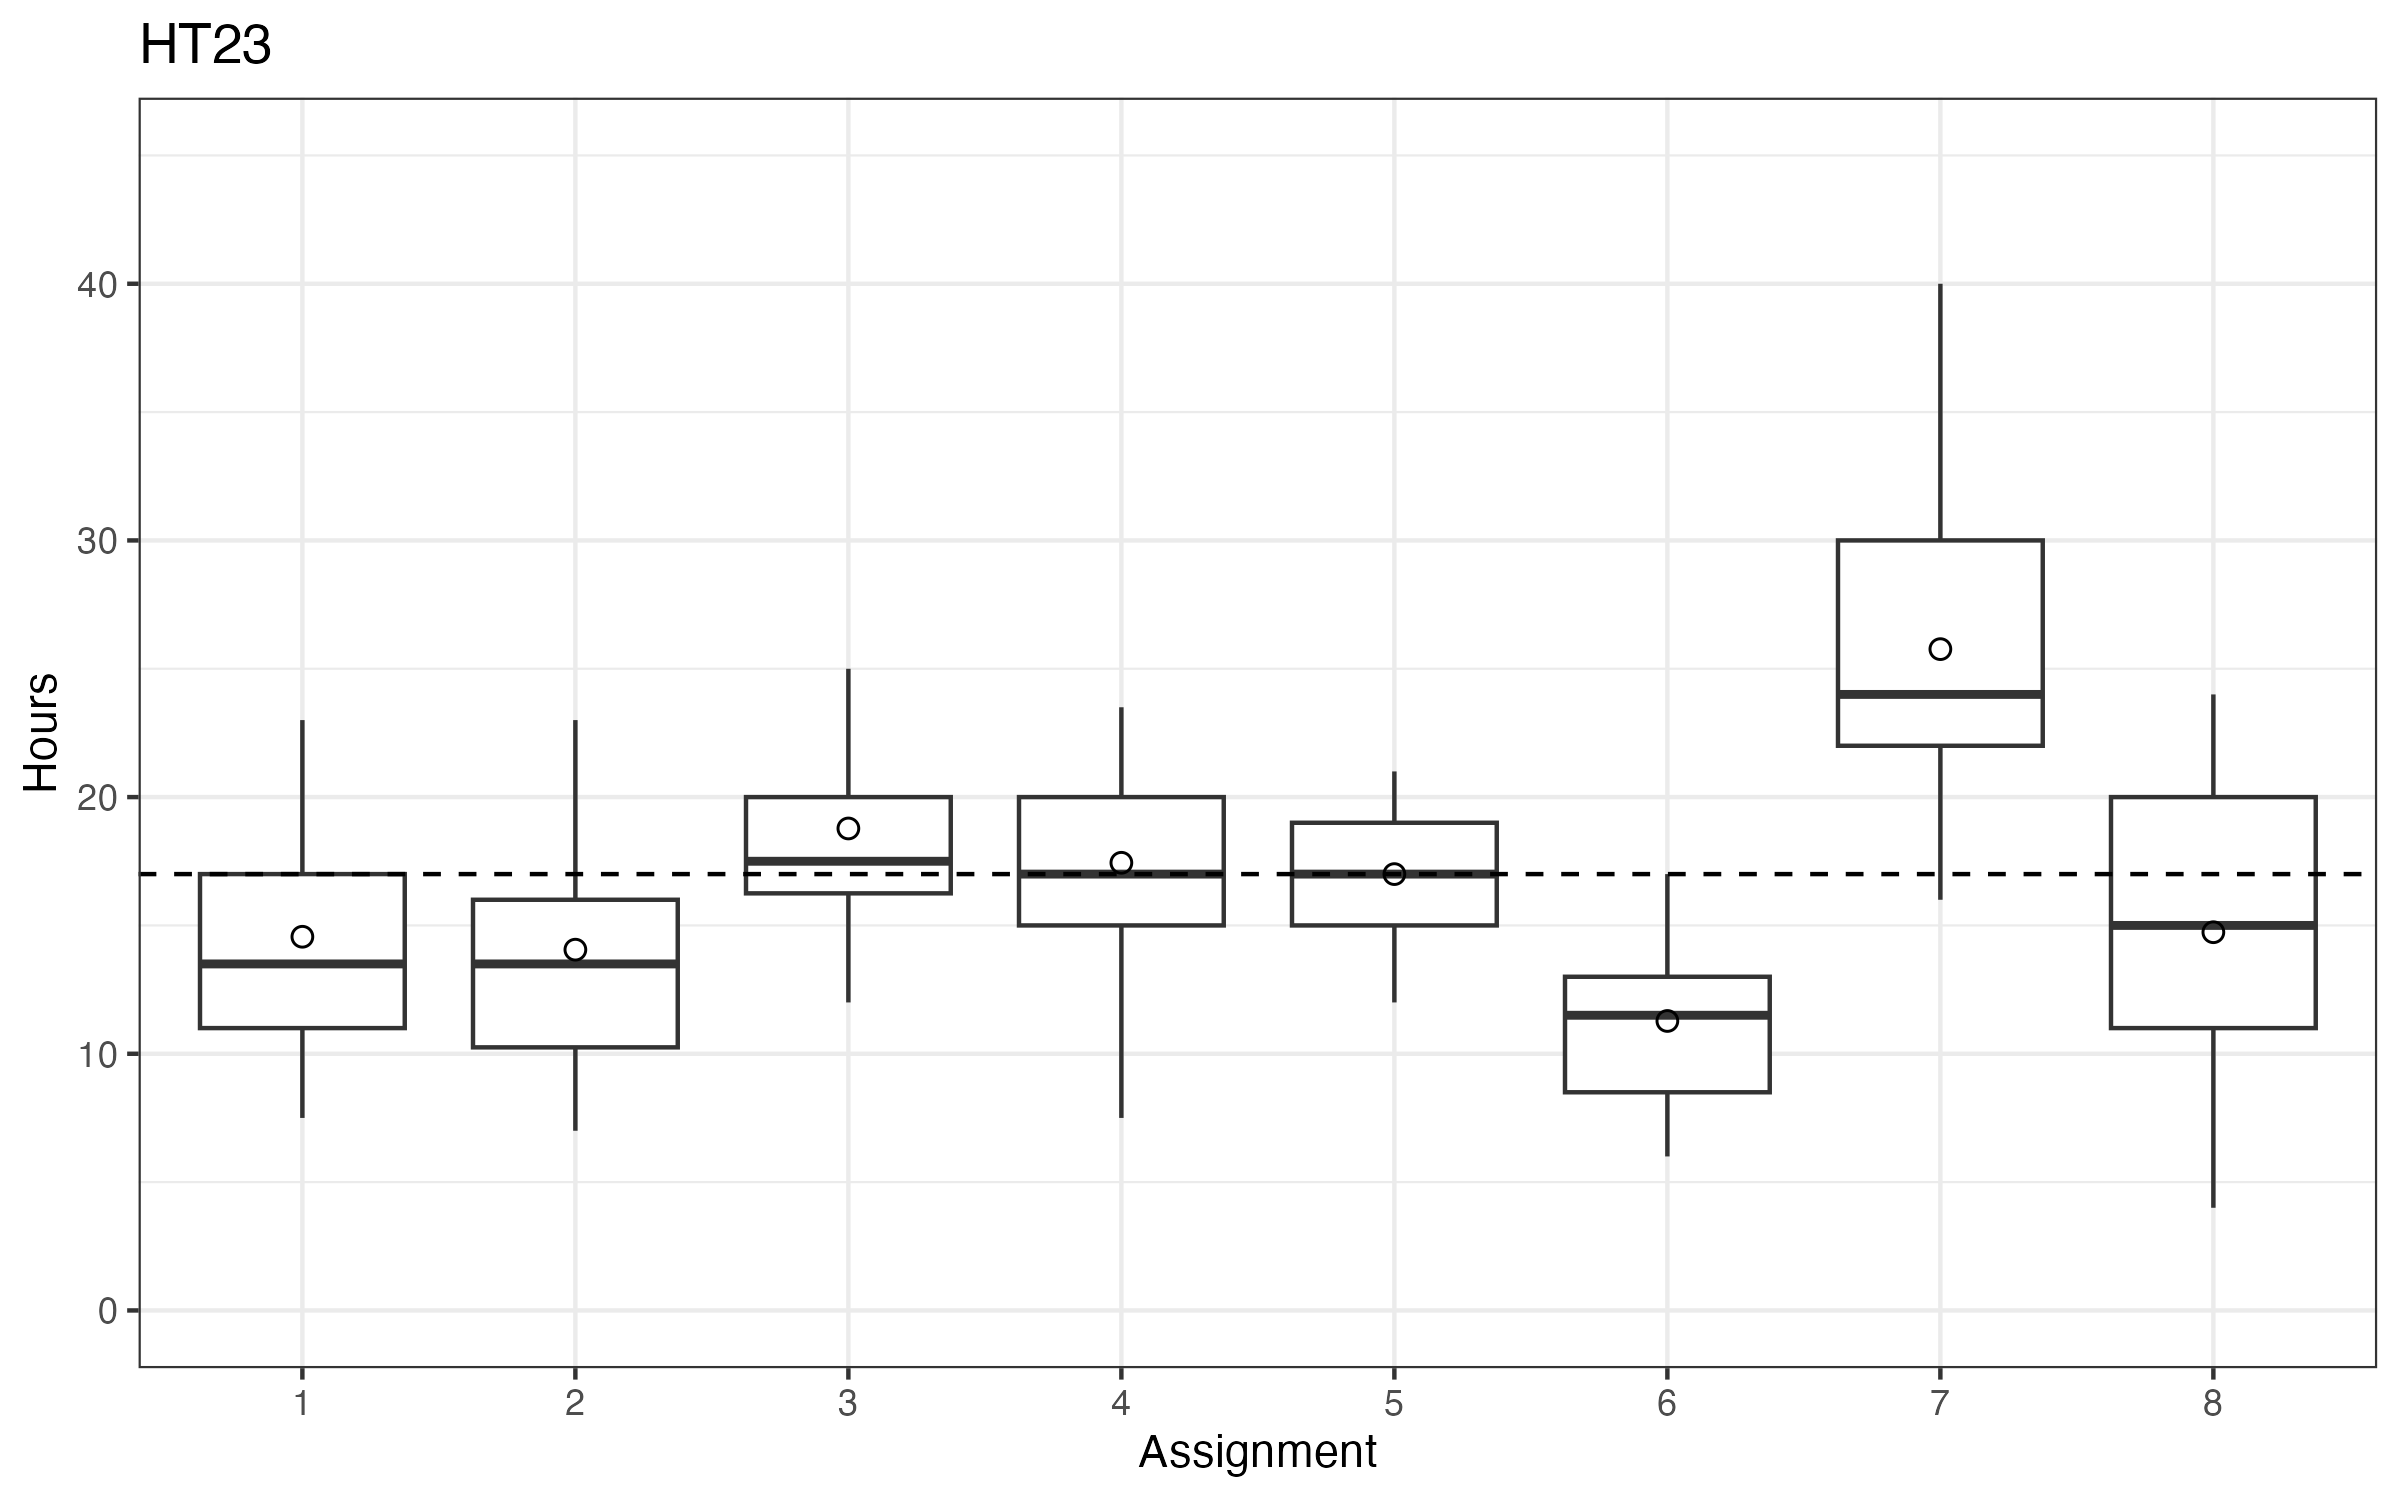
\includegraphics[width=7cm]{figs/time_spent.png}\\
  Student course workload
\end{itemize}

\end{frame}


\begin{frame}{Stan}

\begin{itemize}
  \item Stan is a probabilistic programming framework (PPF) and ecosystem
  \item 40+ developers, 100+ contributors, 100K+ users
  \item R, Python, Julia, Scala, Stata, Matlab, command line interfaces
  \item More than 120 R packages using Stan
  \item Many packages to support diagnostics and workflow
  \item Can be used for frequentist inference as well
  \item Alternative PPF exists, Turing (Julia), Pyro (PyTorch), etc.
  \center
  \vspace{\baselineskip}
  \includegraphics[width=2.5cm]{figs/stan_logo_wide.png}\\
  mc-stan.org
\end{itemize}

\end{frame}

\section{Mini-project}
\frame{\sectionpage}

\begin{frame}{Mini-project}

\begin{itemize}
\item See project instructions on webpage for details.
\item Data analysis of choice on real data.
\item 2-3 students.\pause
\item Supply a half-page project proposal of data and problem in the middle of the course.\pause
\item Ideally, use a model not presented in this course.
\item Project will last two weeks (half time) - but start earlier.
\item The project should use Stan.
\item Approximate 40 hours of work \emph{per student}.\pause
\item The project should result in a 4 page report (PDF) using the ICML LaTeX template (see course page).
\item Project oral presentation (10-15 minutes)
\end{itemize}
\end{frame}


\section{Practicalities}
\frame{\sectionpage}

\begin{frame}{Practicalities}

\begin{itemize}
\item Course page/content: Github -- please do a PR if something is wrong!\pause
\item Communication: Studium\pause
\item Schedule: Time Edit/Studium
\item Assignments submissions: Studium\pause
\item Acknowledgements: Aki Vehtari\pause
\item Teaching assistant: Väinö Yrjänäinen
\end{itemize}

\end{frame}

\begin{frame}{Literature}

\begin{itemize}
  \item Book: Gelman, Carlin, Stern, Dunson, Vehtari \& Rubin: Bayesian Data Analysis, Third Edition. {\footnotesize (online pdf available)}
  \begin{center}
    \includegraphics[width=2.6cm]{figs/BDA3.jpg}
  \end{center}
  \item Additional articles and blog posts (see reading list per week)
\end{itemize}

\end{frame}

\section{Examination}
\frame{\sectionpage}


\begin{frame}{Examination}

\begin{enumerate}
\item To pass (G): All labs, mini-project, and project review need to be passed\pause
\item To pass with distinction (VG): 7/10 VG points\pause
\item If everything is correct in an assignment (>90\%), 1 VG point is awarded \emph{on the first submission deadline}.\pause
\item The mini-project is worth 2 VG-points (if it is passed with distinction).
\item Ph.D. students: I suggest you get VG to pass the course. Make the project a potential paper.
\item Reassesment of grades (supply form to course admin)
\item Failing the course: You will need to redo all assignments and mini-project.
\item Large language models, e.g. chatGPT, are \uured{not allowed}.
\end{enumerate}

\end{frame}

\section{Course improvements}
\frame{\sectionpage}

\begin{frame}{Course improvements since last time}

\begin{itemize}
\item Three step project
\item Improving assignment balance
\end{itemize}

\end{frame}


\frame{\sectionpage}

\begin{frame}{Comments from previous students}

\begin{itemize}
\item Be ready to put the work in!
\item Don’t be afraid to ask questions.
\item Try complete all the assignment on time.
\end{itemize}

\end{frame}


\begin{frame}<handout:0>{Questions?}
Questions?
\end{frame}

%%%%%%%%%%%%%%%%%%%%%%%%%%%%%%%%%%%%%%%%%%%%%%%%%%%%%%%%%%%%%%%%%%




\end{document}


